\chapter{Background}

Drug discovery is an expensive and long-term business. It takes US\$1.8 billion over a period of 13.5 years to develop a new drug \citep{716}. Figure \ref{fig:NewDrugApprovals} \citep{686} shows that in 2009 alone, only 24 new drugs were approved for marketing in the United States, well below the level required to secure the future of the pharmaceutical industry, which has been struggling with decreasing approval numbers for more than a decade. This is particularly remarkable because the level of investment in pharmaceutical R\&D (Research and Development) has dramatically increased by 12\% on average year-on-year since 1970 and at present to about US\$46 billion per year. Therefore drug discovery is economy driven \textit{per se}. Complementing expensive laboratory experiments with low-cost computer simulations is obviously the right way to go.

\begin{figure}
\centering
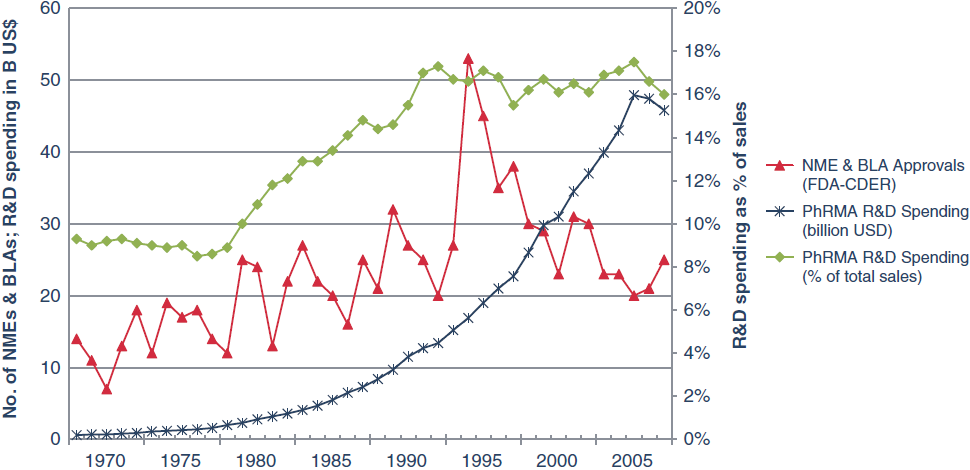
\includegraphics[width=\textwidth]{Background/NewDrugApprovals.png}
\caption{New drug approvals and R\&D investments by PhRMA-member companies from 1970 to 2009. Figure reprinted from \citep{686}.}
\label{fig:NewDrugApprovals}
\end{figure}

\section{Protein-Ligand Docking}

Protein-ligand docking is an essential ingredient of computer-aided drug discovery. It tries to find inhibitors of viral proteins. Take the HIV virus for example (Figure \ref{fig:HIV} \citep{296}). The virus comprises several protein enzymes, which play an important role in replication. In infected cells, the viral reverse transcriptase reversely transcribes viral RNA into viral DNA. The viral integrase integrates viral DNA into human genomic DNA. The viral protease assemblies viral RNA and viral proteins into a new mature virus. If the viral proteins are inhibited, the replication cycle will be blocked. The inhibitors are typically small compounds called ligands. Protein-ligand docking therefore aims to discover inhibitory ligands of pharmaceutical protein targets of therapeutic interest.

\begin{figure}[h]
\centering
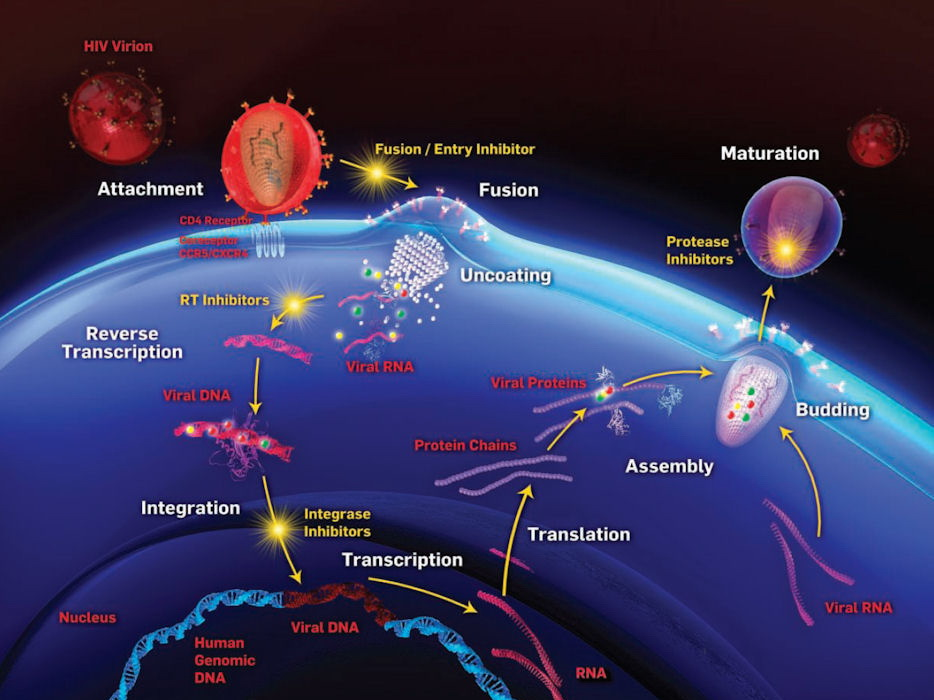
\includegraphics[width=\textwidth]{Background/HIV.jpg}
\caption{Replication cycle of HIV/AIDS. Figure reprinted from \citep{296}.}
\label{fig:HIV}
\end{figure}

Protein-ligand docking is a method which predicts the preferred conformation and binding affinity of a small ligand when bound to a macro protein to form a stable complex. A conformation refers to a vector of position, orientation, and torsions if any (Figure \ref{background:DegreeOfFreedom}). A binding affinity suggests how well the interactions formed between the ligand and the protein. Empirically speaking, it is the overall effect of various chemical interactions involved, such as van der Waals force, electrostatic force, hydrogen bonding, hydrophobic interactions, stack interactions, and the like. Virtual screening can be regarded as a massive version of docking. Instead of docking one single ligand, it docks a database of drug-like ligands to a viral protein of interest, ranks them according to their predicted binding affinity, and shortlists the best ones for further investigation.

\begin{figure*}
\centering
\subfloat[Positional degree of freedom.]
{
  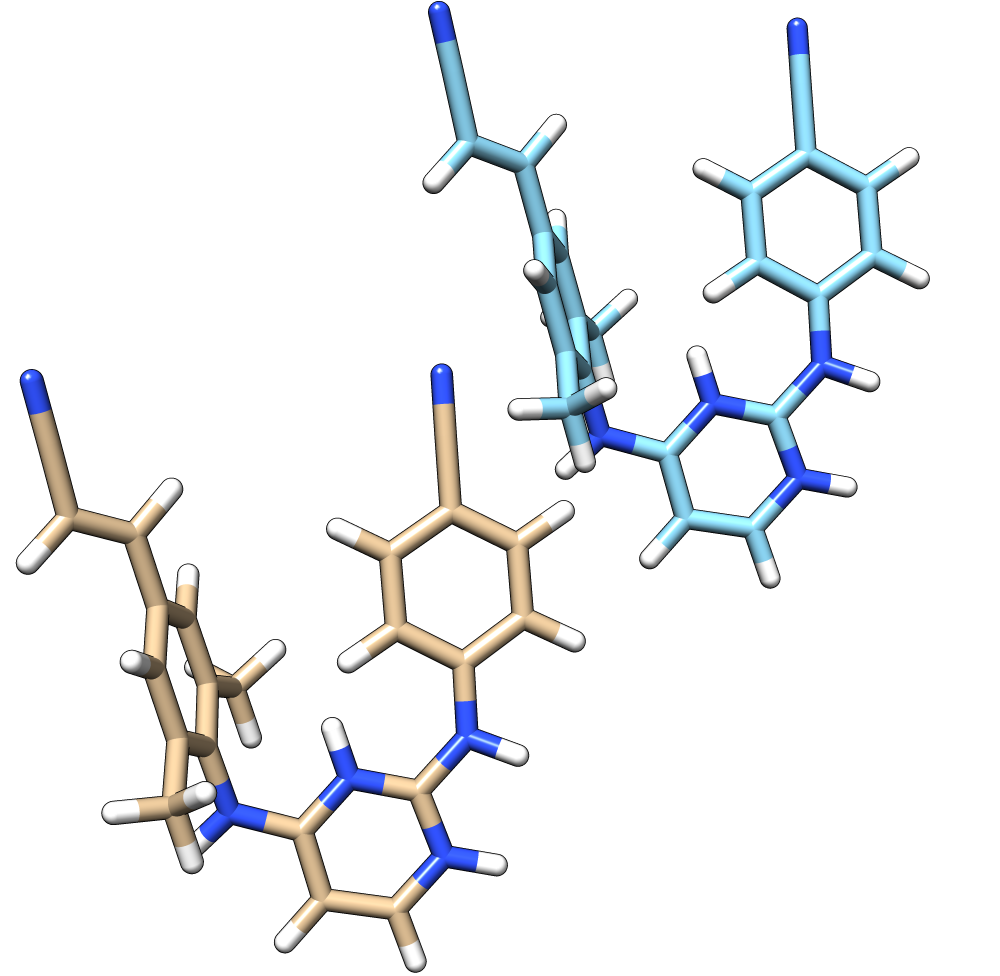
\includegraphics[width=0.32\linewidth]{Background/PositionalDOF.png}
}
\subfloat[Orientational degree of freedom.]
{
  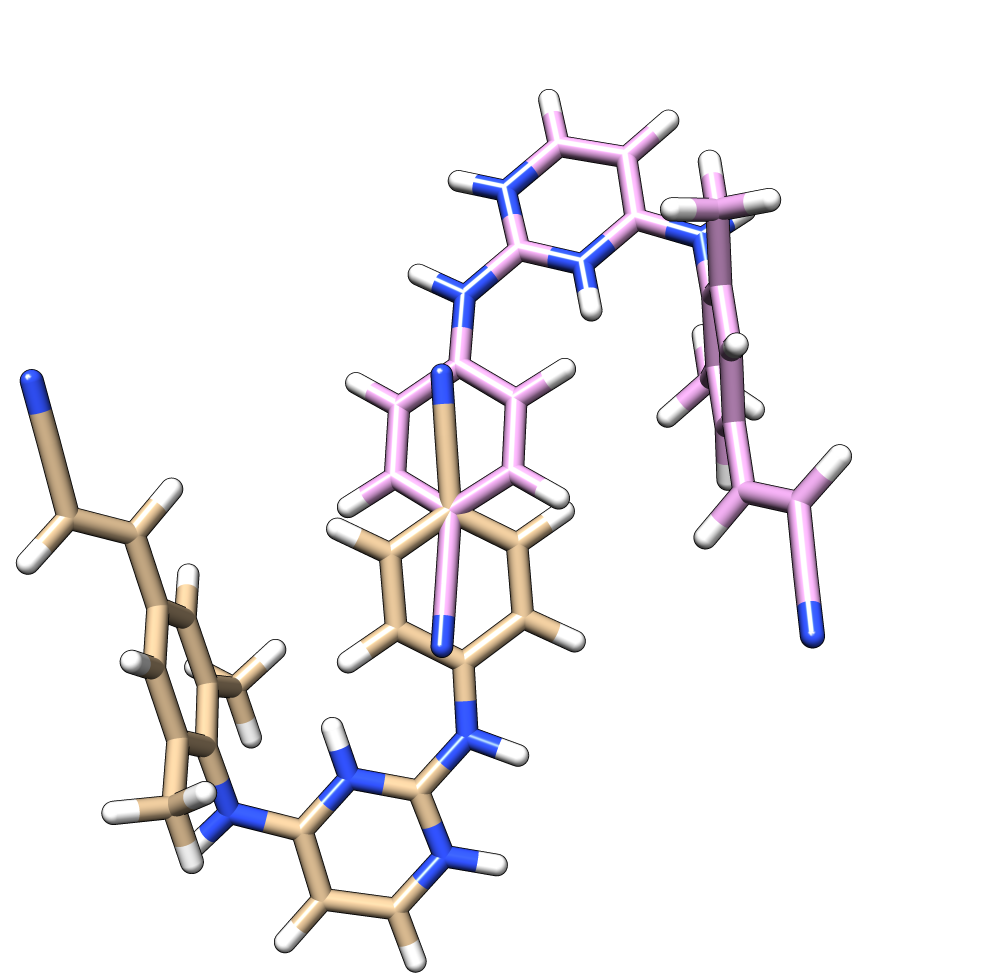
\includegraphics[width=0.32\linewidth]{Background/OrientationalDOF.png}
}
\subfloat[Torsional degree of freedom.]
{
  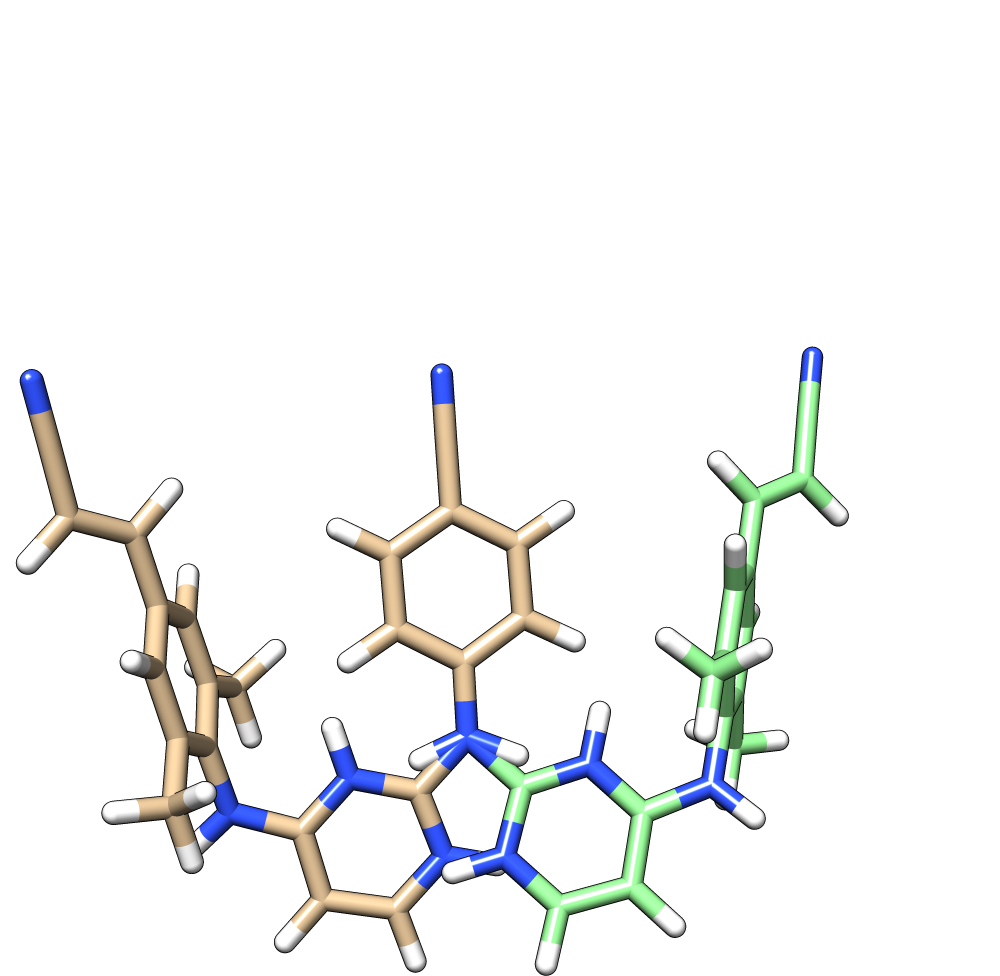
\includegraphics[width=0.32\linewidth]{Background/TorsionalDOF.png}
}
\caption{Positional, orientational and torsional degree of freedom.}
\label{background:DegreeOfFreedom}
\end{figure*}

Treating a docking program as a black box, its input includes the 3D structures of a protein and a ligand, while its output includes several predicted conformations and their predicted binding affinity. For the protein input, thanks to the rapid evolution of X-ray crystallography and NMR (Nuclear Magnetic Resonance) technologies, more and more 3D structures of biological macromolecules at atomic level have been revealed and deposited into the world's largest repository PDB (Protein Data Bank) \citep{540,537}. As of 4 Sep 2012, there are 84,381 structures in PDB. For the ligand input, the ZINC database \citep{532,1178} contains over 21 million purchasable compounds in ready-to-dock, 3D formats. The TCM@Taiwan database \citep{528} is the world's largest and most comprehensive free down small molecular database on traditional Chinese medicine. In addition, the PubChem database \citep{526} is a public repository for biological properties of small molecules, containing biological test results for more than 700,000 compounds. The PDBbind database \citep{529,530} and the CSAR NRC HiQ Set \citep{857,960} are collections of binding affinities for protein-ligand complexes with known 3D structures. The refined set of PDBbind v2011 and the two sets of CSAR NRC HiQ Set 24Sept2010 comprise 2,455 and 343 protein-ligand complexes respectively, with experimentally determined binding affinity data. For the output, PyMOL \citep{1221}, Chimera \citep{1219}, VMD \citep{1220}, AutoDockTools4 \citep{596}, ViewDock TDW \citep{559}, PoseView \citep{748} and LigPlot+ \citep{951} can be used to visualize docked conformations and plot putative interaction charts. AuPosSOM \citep{598} can be used to cluster docked conformations. BEDROC \citep{490} and SLR \citep{489} can be used as statistical metrics for docking method evaluation.

Treating a docking program as a white box, it consists of two typical components, an algorithm to explore the conformational space of the ligand and the protein, and a scoring function to predict binding affinity given a conformation. Over recent decades, dozens of docking programs have been developed, such as DOCK \citep{1222}, AutoDock 4 \citep{785,596}, AutoDock Vina \citep{595}, QuickVina \citep{1193}, PLANTS \citep{610,607,779}, FITTED \citep{602}, CDOCK \citep{1224}, and CRDOCK \citep{1200}. Likewise, dozens of scoring functions have also been developed, such as RF-Score \citep{564}, SFCscore \citep{581}, LISA \citep{775}, and NNScore 2.0 \citep{977}. Refer to survey papers for a more complete list \citep{493,922} and for program comparison \citep{556,637}.

Amongst a sea of docking programs, AutoDock Vina \citep{595} (hereafter Vina for short) is a competitive one. It is free and open source under Apache License 2.0. It has been shown to run faster than its predecessor AutoDock 4 \citep{596} by an order of magnitude when benchmarking on virtual screening for HIV protease inhibitors \citep{556}. Released in the second half of 2010, Vina has been cited over 400 times and adopted by a wide community of researchers. Indeed, it is intensively used in our research projects too. In Vina, the binding affinity is evaluated as free energy. The lower the free energy, the higher the binding affinity. There is a PyMOL plugin for AutoDock and Vina \citep{609}. MOLA is a bootable, self-configuring system for virtual screening using AutoDock4/Vina on computer clusters \citep{773}.

In addition to pure docking program development, there is also a pool of successful case studies of using protein-ligand docking programs to discover novel and potent ligands for pharmacological proteins of therapeutic interest. To name a few, Vina was used for docking studies on the HEPT derivatives of HIV-1 reverse transcriptase \citep{843}, for side-chain residue flexibility study of VEGFR-2 (Vascular Endothelial Growth Factor Receptor 2), a known protein target for anti-angiogenic agents \citep{1084}, and for identification of novel inhibitors of sirtuin 2, a NAD\textsuperscript{+}-dependent histone deacetylase enzyme \citep{1177}. Such exciting success stories prove the real power of protein-ligand docking for computer-aided drug discovery.

\section{Ligand Synthesis}

Given a pharmacological protein of therapeutic interest, protein-ligand docking tries to discover promising ligands out of existing compound databases. Apparently the diversity of its outcome is limited by the diversity of the database. In other words, docking will fail if the selected database contains no promising ligands at all. Hence constructing \textit{de novo} ligands from fragments now becomes a hot research problem.

Figure \ref{igrow:LigandDesign} \citep{363} illustrates two strategies for ligand design, link/grow strategy and lattice strategy. The recent years have seen a prosperity of \textit{de novo} ligand design programs, such as MORPH \citep{365}, GARLig \citep{471}, LEA3D \citep{1223}, LigBuilder 2 \citep{749}, AutoT\&T \citep{780}, AutoGrow \citep{466}, AutoClickChem \citep{1051}, CrystalDock \citep{954}, and LigMerge \citep{1181}. Refer to review papers for a more complete list \citep{363,367,472,1006} and methodology development \citep{470,982}. Meanwhile, several databases have been established for fragment-based drug design, such as e-Drug3D \citep{1125}. Furthermore, a number of compounds that evolved from fragments have entered the clinic, and the approach is increasingly accepted as an additional route to identifying new ligands in inhibitor design \citep{363,367,472,474,1006}.

\begin{figure}[t]
\centering
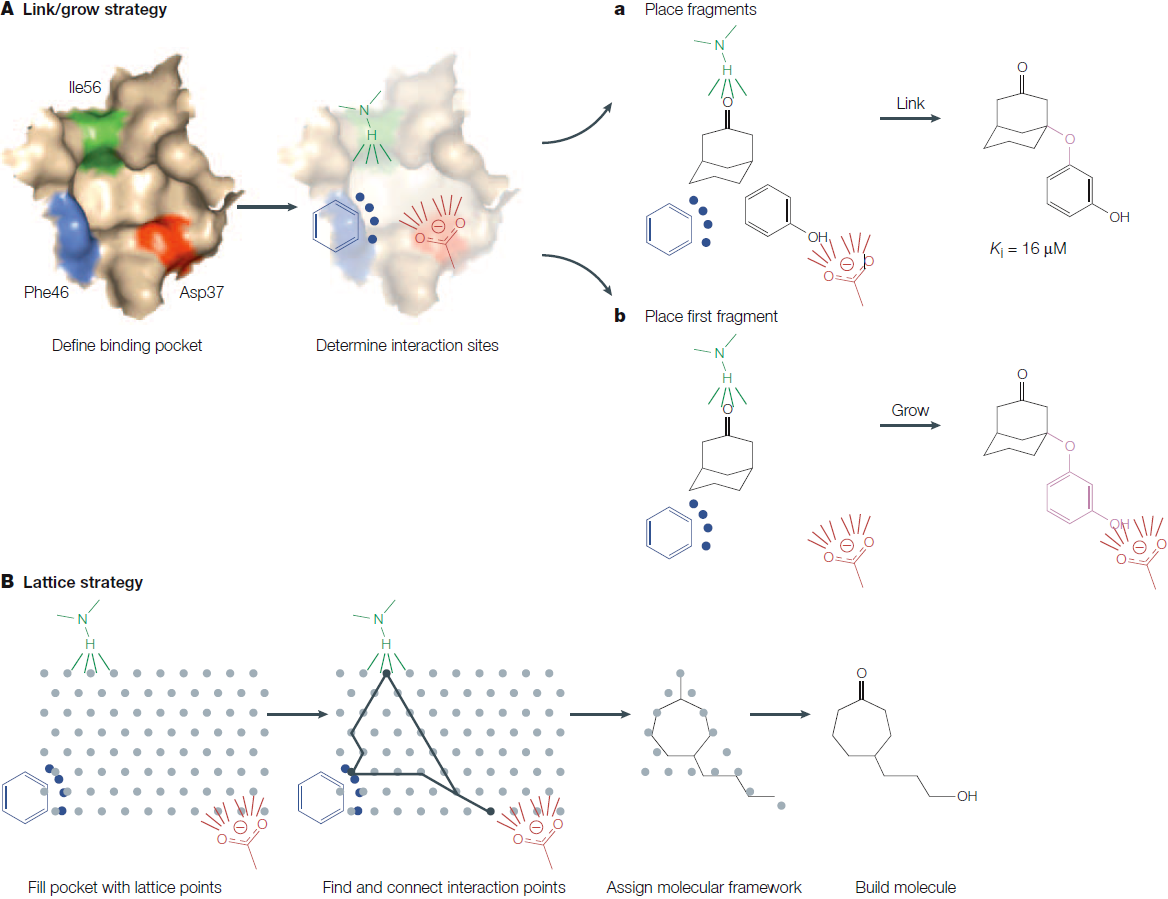
\includegraphics[width=\textwidth]{igrow/LigandDesign.png}
\caption{Ligand design strategies. Figure reprinted from \citep{363}.}
\label{igrow:LigandDesign}
\end{figure}

A computational synthesis program helps to explore a much larger chemical space for novel drugs, but the search space is just too huge, virtually infinite. The number of chemically feasible, drug-like molecules has been estimated to be in the order of 10\textsuperscript{60} to 10\textsuperscript{100} \citep{1104}, from which the most promising candidates have to be selected and synthesized. Hence, rather than systematic construction and evaluation of each individual compound, computational synthesis programs rely on the principle of local optimization, which does not necessarily lead to the globally optimal solution. In fact, most software implementations are non-deterministic, and rely on some kind of stochastic structure optimization.

Amongst the many ligand synthesis programs, AutoGrow \citep{466} is a representative one which implements genetic algorithm to create a population of ligands. It uses Vina \citep{595} as external docking engine for the selection operator. AutoClickChem \citep{1051} is capable of performing \textit{in silico} click chemistry reactions, ensuring that chemical synthesis is fast, cheap, and comparatively easy for subsequent testing in biochemical assays. LigMerge \citep{1181} is an automated, ligand-based algorithm for systematically swapping the chemical moieties of known ligands to generate novel ligands with potentially improved potency. It has been shown to identify compounds predicted to inhibit peroxisome proliferator-activated receptor gamma, HIV reverse transcriptase, and dihydrofolate reductase with affinities higher than those of known ligands. The above three programs are free and open source. They are used as baseline tools in our research projects.

\section{Software as a Service}

SaaS (Software as a Service) is part of the nomenclature of cloud computing. It is a software delivery model in which software and associated data are centrally hosted on the cloud. SaaS is typically accessed by users using a thin client via a web browser. In computational biology, ten simple rules have been summarized for providing a scientific web resource \citep{677}. Software and web sites do count for getting ahead as a computational biologist \citep{260}.

Up to date, several SaaS platforms for protein-ligand docking or ligand synthesis have been created. DOCK Blaster \citep{557} investigates the feasibility of full automation of protein-ligand docking. It utilizes DOCK \citep{1222} as the docking engine and ZINC \citep{532,1178} as the ligand database. iScreen \citep{899} is a compacted web server for TCM (Traditional Chinese Medicine) docking and followed by customized \textit{de novo} drug design. It utilizes PLANTS \citep{610,607,779} as the docking engine and TCM@Taiwan \citep{528} as the ligand database. It also utilizes LEA3D \citep{1223} for \textit{de novo} ligand design. FORECASTER \citep{1012} is a web interface consisting of a set of tools for the virtual screening of small molecules binding to biomacromolecules (proteins, receptors, and nucleic acids). It utilizes the flexible-target docking program FITTED \citep{602} as docking engine. VSDMIP \citep{848} is an automated structure- and ligand-based virtual screening platform with a PyMOL graphical user interface. It utilizes CDOCK \citep{1224} as the docking engine.

\section{General-Purpose Computing on GPU}

The modern GPU (Graphics Processing Unit) has evolved from a fixed-function graphics pipeline to a programmable parallel processor with extremely high computational throughput and tremendous memory bandwidth at an affordable price. Performance evaluation of hybrid programming patterns for large CPU/GPU heterogeneous clusters has been carried out \citep{1035}. The past five years have seen a fruitful of algorithms for computer-aided drug discovery being ported to the GPU and gaining orders of magnitude of speedup over single threaded CPU counterparts. To name a few, such GPU-accelerated applications include FTMap \citep{722} for binding site mapping, CUDASW++2.0 \citep{189} for protein database search, the leader and the spread algorithms \citep{750} for compound selection, PIPER \citep{723}, PLANTS \citep{779} and parallelized AutoDock \citep{696} for molecular docking, SIML \citep{726} and Tanimoto matrix calculation \citep{881} for chemical similarity calculation, OpenMM \citep{373} and MD-GPU \citep{374} for molecular dynamics, PAPER \citep{491} for molecular shape comparison, CAMPAIGN \citep{932} for data clustering, and visualization \citep{986}.

As of September 2012, NVIDIA’s latest GPU architecture is codenamed ``Kepler" with its full implementation codenamed ``GK104", while AMD's latest GPU architecture is codenamed ``Southern Islands" with its full implementation codenamed ``Tahiti".

\subsection{NVIDIA GK104 and CUDA}

From the hardware perspective, the GK104-based GeForce GTX 680 GPU features 3.09 TFLOPS single-precision computing power and 128 GFLOPS double-precision computing power, 2GB GDDR5 memory with a bandwidth of 192GB/s, and a TDP (Thermal Design Power) of 195W.

Figure \ref{GPU:GeForceGTX680BlockDiagram} shows the block diagram of GeForce GTX 680, which consists of 4 GPCs (Graphics Processing Clusters), each having a dedicated raster engine and 2 SMX (next-generation Streaming Multiprocessors) units. With a total of 8 SMX units, the GeForce GTX 680 has 1536 CUDA Cores.

\begin{figure}
\centering
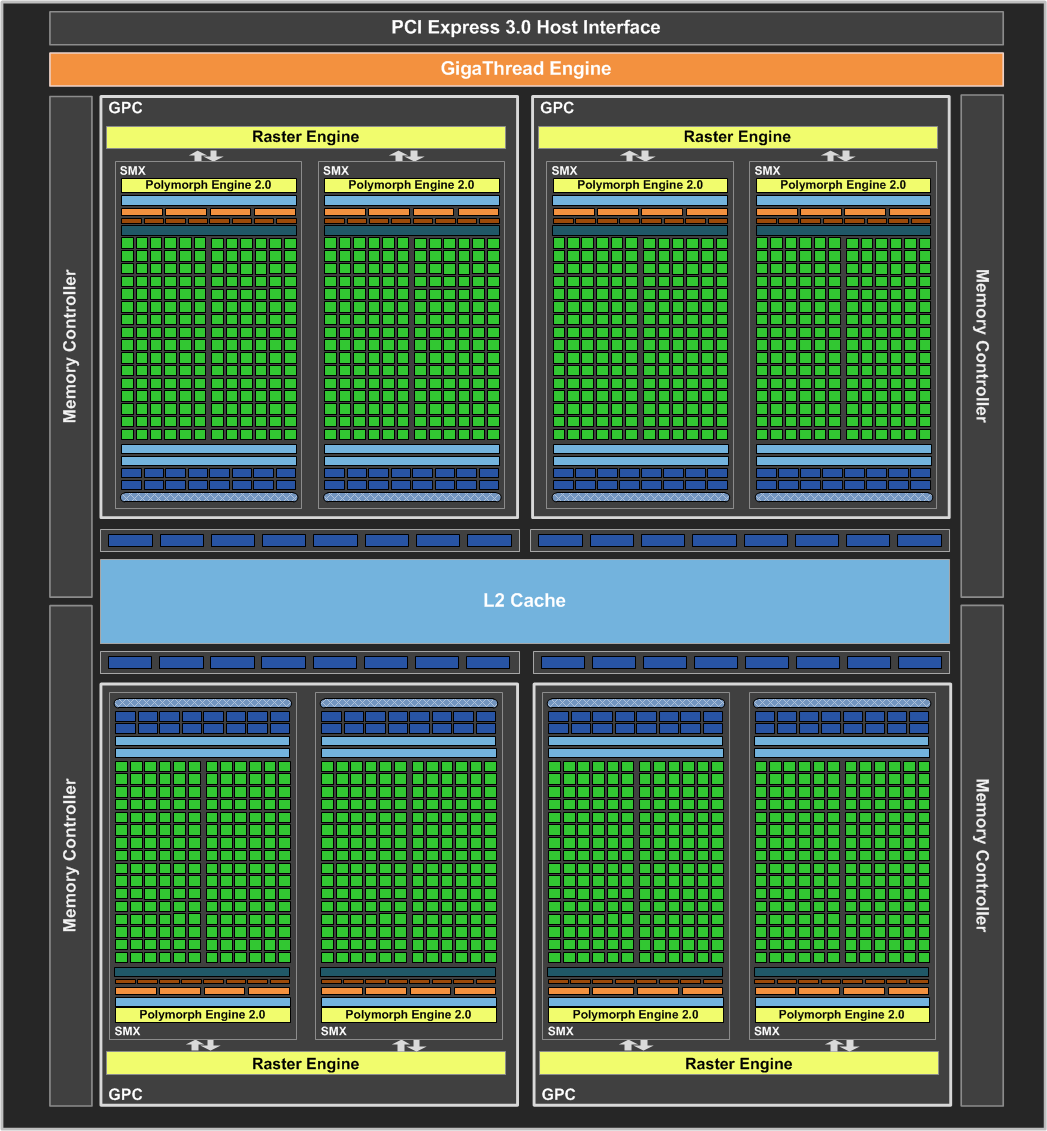
\includegraphics[width=\textwidth]{GPU/GeForceGTX680BlockDiagram.png}
\caption{NVIDIA GeForce GTX680 block diagram. Source: NVIDIA.}
\label{GPU:GeForceGTX680BlockDiagram}
\end{figure}

Figure \ref{GPU:GeForceGTX680SMX} shows the block diagram of GK104 SMX unit, which features 192 IEEE 754-2008 compliant single-precision CUDA cores, 32 SFUs (Special Function Units), 4 warp schedulers, 8 instruction dispatch units, and 64KB of configurable shared memory / L1 cache. Each CUDA core has fully pipelined floating-point and integer arithmetic logic units, while the SFUs handle fast approximate transcendental and graphics interpolation instructions.

The SMX schedules threads in groups of 32 parallel threads called warps. The 4 warp schedulers allow 4 warps to be issued and executed concurrently. Each warp scheduler is capable of dispatching 2 instructions per warp every clock in order to feed the execution resources of SMX.

\begin{figure}
\centering
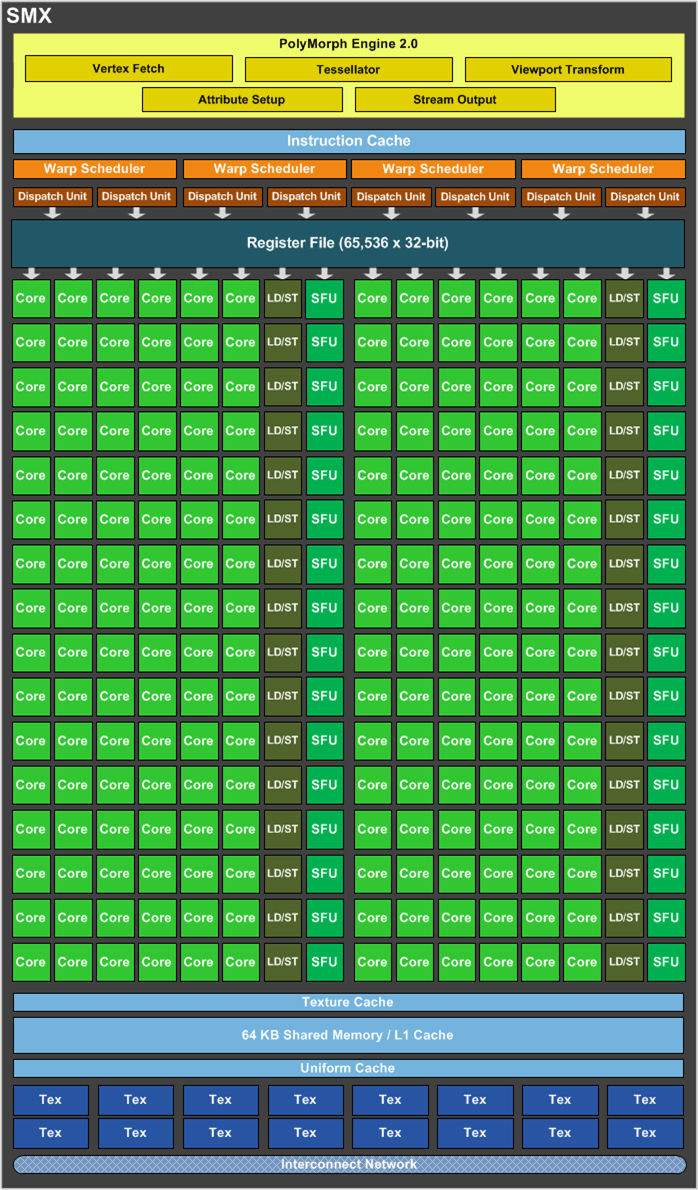
\includegraphics[width=\textwidth]{GPU/GeForceGTX680SMX.png}
\caption{NVIDIA GeForce GTX680 SMX. Source: NVIDIA.}
\label{GPU:GeForceGTX680SMX}
\end{figure}

From the software perspective, the GeForce GTX 680 supports CUDA (Compute United Device Architecture), and thus can execute programs written in C, C++, Fortran, and other languages. A CUDA program invokes functions called kernels that execute across parallel CUDA threads, which are organized into thread blocks and grids of thread blocks. The hierarchy of CUDA threads maps to the hierarchy of CUDA cores on the GPU; a GPU executes one or more grids; an SMX executes one or more thread blocks; and CUDA cores and other execution units in the SMX execute thread instructions from kernel compilation.

Figure \ref{GPU:CUDAMemoryHierarchy} shows the CUDA hierarchy of threads, blocks and grids, and their corresponding memory space. A CUDA thread within a thread block maintains a program counter and executes an instance of the kernel. It has a per-thread private memory space used for register spills, function calls, and C automatic array variables. A thread block is a set of concurrently executing threads that can cooperate among themselves through barrier synchronization and shared memory. It has a per-block shared memory space used for inter-thread communication, data sharing, and result sharing. A grid is an array of thread blocks that execute the same kernel, read inputs from global memory, write results to global memory, and synchronize between dependent kernel calls. Grids share results in global memory after kernel-wide synchronization.

\begin{figure}
\centering
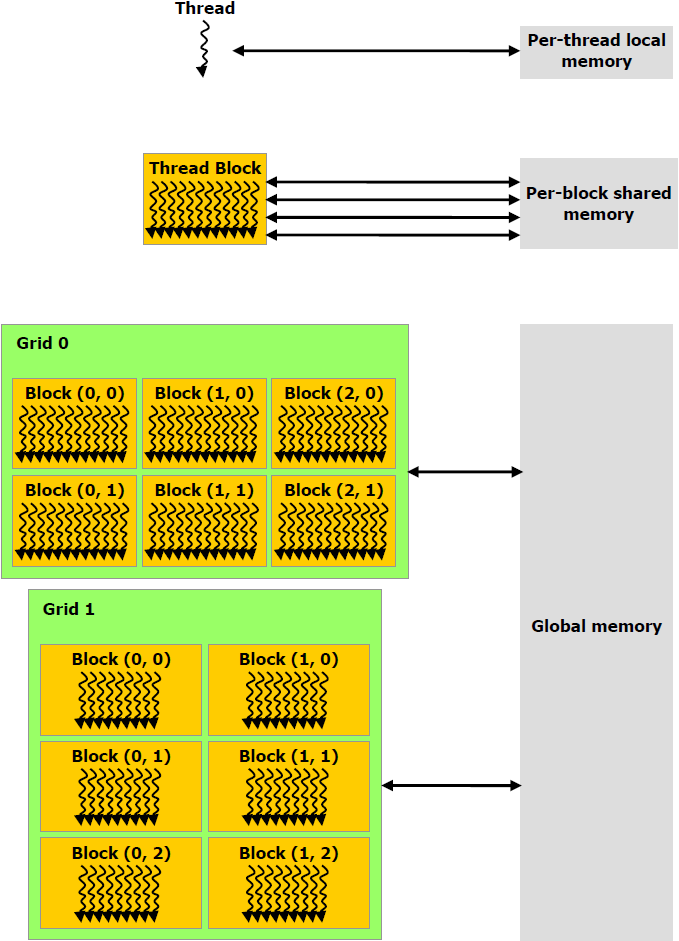
\includegraphics[width=\textwidth]{GPU/CUDAMemoryHierarchy.png}
\caption{CUDA hierarchy of threads, blocks, and grids, with corresponding per-thread private, per-block shared, and per-application global memory spaces. Source: NVIDIA.}
\label{GPU:CUDAMemoryHierarchy}
\end{figure}

\subsection{AMD Tahiti and OpenCL}

From the hardware perspective, the Tahiti-based Radeon HD 7970 GPU features 3.79 TFLOPS single-precision computing power and 947 GFLOPS double-precision computing power, 3GB GDDR5 memory with a bandwidth of 264GB/s, and a TDP of 250W.

Figure \ref{GPU:RadeonHD7970BlockDiagram} shows the block diagram of Radeon HD 7970, which consists of 32 GCN (Graphics Core Next) cores, each heaving 64 stream processors, translating to a total of 2048 stream processors.

\begin{figure}[t]
\centering
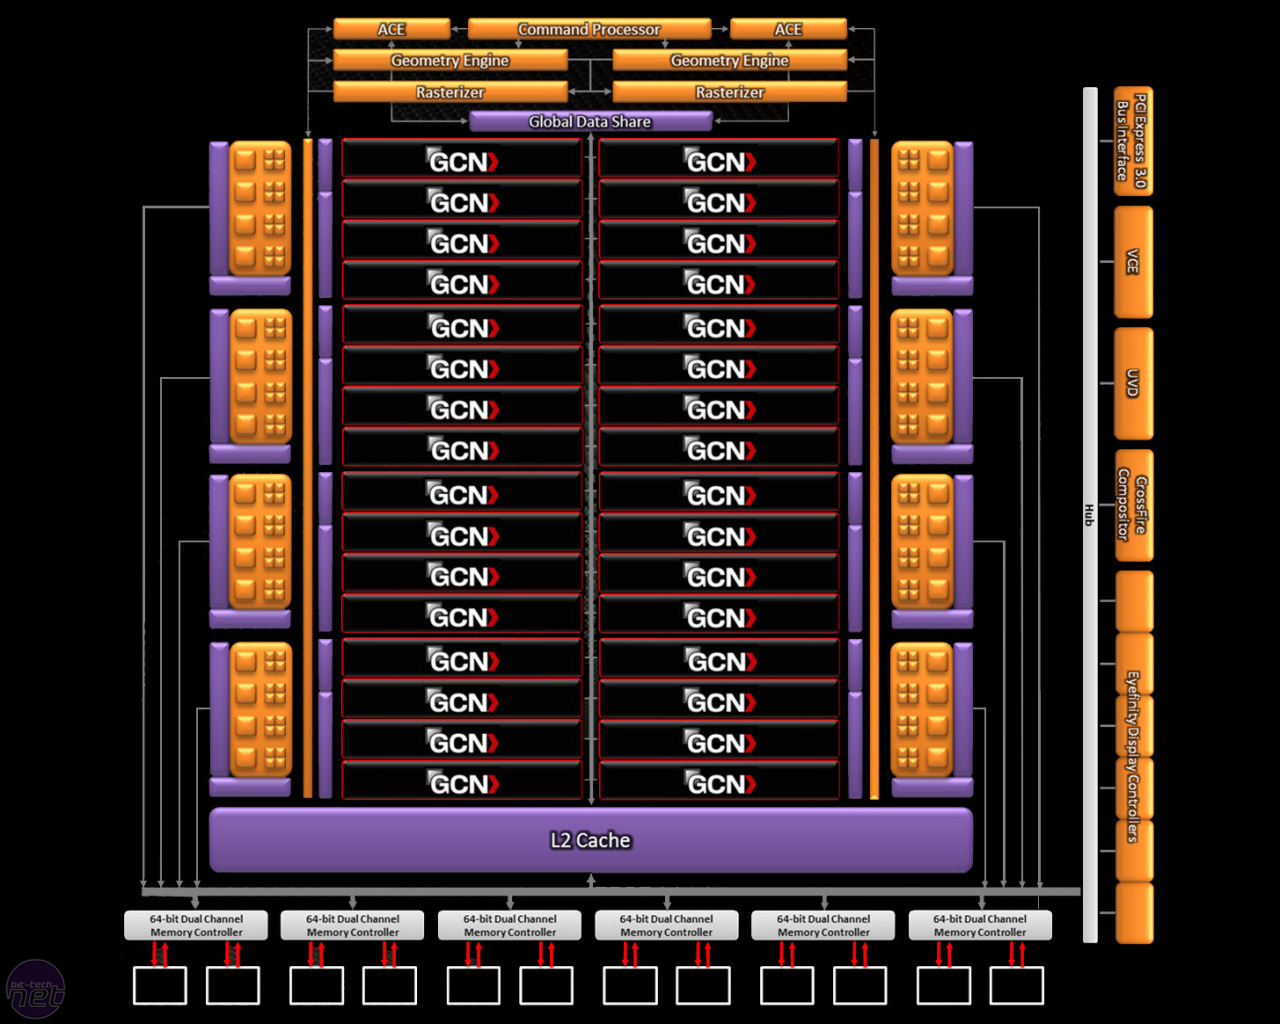
\includegraphics[width=\textwidth]{GPU/RadeonHD7970BlockDiagram.jpg}
\caption{AMD Radeon HD 7970 block diagram. Source: AMD.}
\label{GPU:RadeonHD7970BlockDiagram}
\end{figure}

Figure \ref{GPU:RadeonHD7970GCN} shows the block diagram of a GCN core, which features a scheduler, 4 SIMD-16 vector units, 4 64KB vector registers, a single scalar unit, 64KB of LDS (Local Data Share), and 16KB of L1 cache. The GCN core schedules threads in groups of 16 parallel threads called wavefronts. The 4 SIMD-16 vector units are capable of not only processing 4 wavefronts in 4 clock cycles, equivalent to one wavefront per cycle, but also handling special functions like transcendentals at a rate of 4 operations per clock cycle. The scalar unit assists with flow control and handles address generation for pointers. The L1 cache has an aggregate bandwidth of about 2 TB/s.

\begin{figure}
\centering
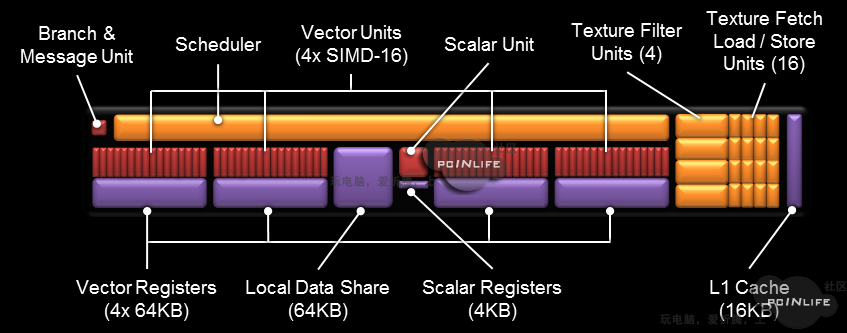
\includegraphics[width=\textwidth]{GPU/RadeonHD7970GCN.png}
\caption{AMD Radeon HD 7970 GCN. Source: AMD.}
\label{GPU:RadeonHD7970GCN}
\end{figure}

Figure \ref{GPU:RadeonHD7970CacheHierarchy} shows the cache hierarchy of Radeon HD 7970. A group of 4 GCN cores shares a 16KB instruction cache and a 32KB scalar data cache. The GDS (Global Data Share) enables L1 cache synchronization across all the GCN cores, which communicate over a shared bus to 6 128KB L2 cache partitions, each associated with a 64-bit dual-channel memory controllers, for a total of 768KB of L2 cache. The L2 cache can transfer nearly 710GB/s at 925MHz.

\begin{figure}
\centering
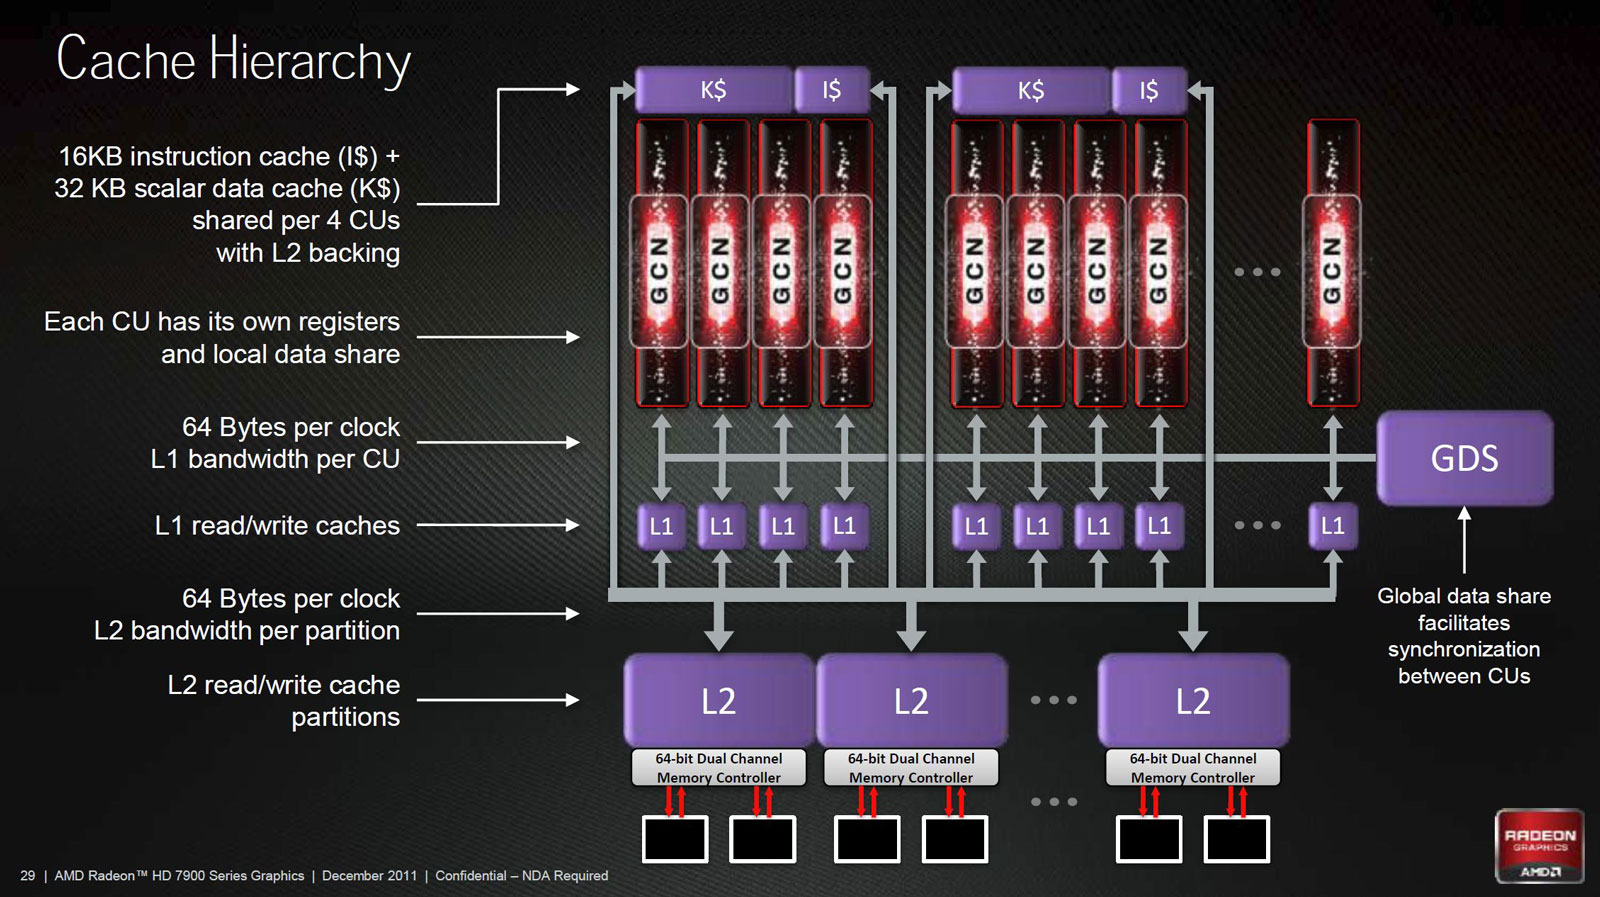
\includegraphics[width=\textwidth]{GPU/RadeonHD7970CacheHierarchy.jpg}
\caption{AMD Radeon HD 7970 cache hierarchy. Source: AMD.}
\label{GPU:RadeonHD7970CacheHierarchy}
\end{figure}

From the software perspective, the Radeon HD 7970 supports OpenCL (Open Computing Language) 1.2, and thus can execute programs written in C. There is a C++ wrapper for OpenCL 1.1. An OpenCL program invokes functions called kernels that execute across parallel work-items, which are organized into work-groups. The hierarchy of work-items maps to the hierarchy of stream processors on the GPU; a GPU executes one or more kernels; a GCN core executes one or more work-groups; and stream processors execute work-item instructions from kernel compilation.

Portability is the distinct feature that distinguishes OpenCL from CUDA. Multiple conformant implementations of OpenCL from AMD, NVIDIA, Intel, IBM, ARM, and embedded device vendors are shipping, fulfilling the philosophy of ``write once, execute everywhere".

\chapterend
